\documentclass[10pt, a4paper]{article} 
\usepackage[
a4paper,
left=2cm,      
right=2cm,     
top=3cm,     
bottom=3cm,    
headheight=10em 
]{geometry}
\usepackage[utf8]{inputenc}
\usepackage{amsmath,amsthm,amssymb,xfrac}
\usepackage{fancyhdr}
\usepackage[hungarian]{babel}
\usepackage{graphicx}
\usepackage{float}
\usepackage{comment}
\usepackage{natbib}
\usepackage{empheq}
\usepackage{wrapfig}
\usepackage{chngcntr}
\usepackage{physics}
\usepackage{mathtools}
\counterwithin{figure}{section}
\usepackage{titlesec}
\usepackage{dsfont}
\usepackage{pdfpages}
\usepackage{t1enc}
\usepackage{tabto}
\usepackage{pgfplots}
\graphicspath{ {./images/} }
\usetikzlibrary{arrows}
\usetikzlibrary{patterns}
\setlength{\marginparwidth}{0pt}
\setlength{\marginparsep}{0pt}

\pagestyle{fancy}
\fancyhf{}
\cfoot{\thepage. oldal}
\lhead{
	\textbf{Dinamika 1. Házi feladat}
	\\Kindlik Dániel
	\tabto{400pt}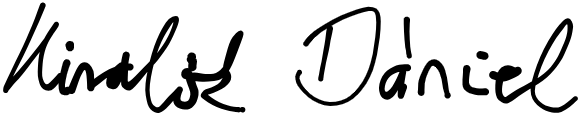
\includegraphics[width=80pt]{ alairas.png }
	\\AHU27Z
	}
	
\newcounter{feladatcounter}
\newcommand{\feladat}{
	\stepcounter{feladatcounter}
	\begin{trivlist}
		\item[\hskip \labelsep {\bfseries
			{\arabic{feladatcounter}. Feladat:}}]\end{trivlist}}
\newcommand{\adat}{\begin{trivlist}\item[\hskip \labelsep {\bfseries 
			{Adatok:}}]\end{trivlist}}
\setlength{\parskip}{0.22em} 

\newcommand{\rads}{\;\mathrm{\left[rad/s\right]}}
\newcommand{\radss}{\;\mathrm{\left[rad/s^2\right]}}
\newcommand{\ms}{\;\mathrm{\left[m/s\right]}}
\newcommand{\mss}{\;\mathrm{\left[m/s^2\right]}}
\newcommand{\meter}{\;\mathrm{\left[m\right]}}
\newcommand{\mm}{\mathrm{\left[mm\right]}}
\newcommand{\dimnel}{\mathrm{\left[-\right]}}
\newcommand{\fok}{\mathrm{^\circ}}
\newcommand{\gpa}{\mathrm{\left[GPa\right]}}
\newcommand{\mpa}{\mathrm{\left[MPa\right]}}
\newcommand{\jpcm}{\mathrm{\left[J/cm^3\right]}}

\begin{document}
	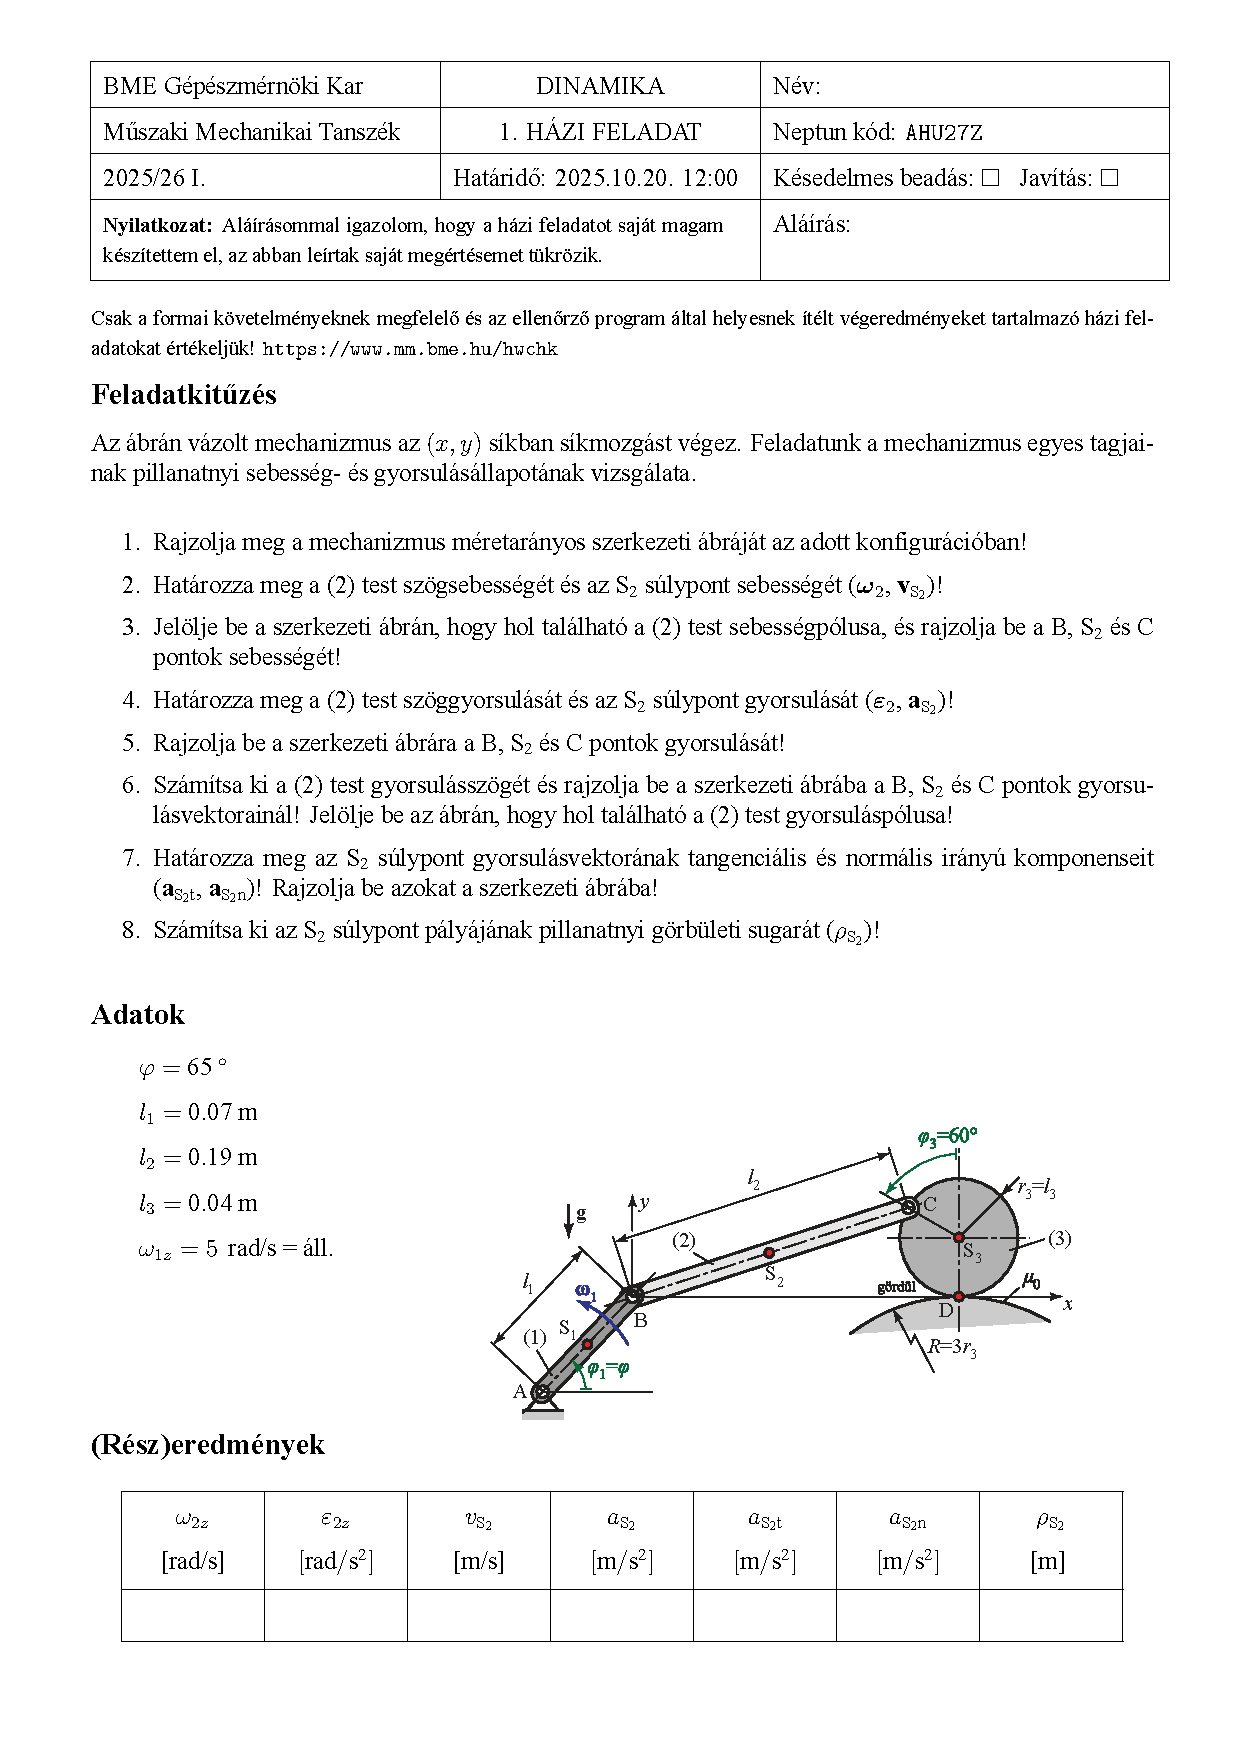
\includepdf{elolap.pdf}
	(A feladatokban levő egyenletrendszereket egy általam készített \textbf{Python} program segítségével oldottam meg, így azoknak csak a megoldása szerepel itt. Emellett a feladathoz szükséges ábrákat \textbf{Latex}-ban a \texttt{tikz} könyvtár segítségével ábrázoltam.)
	\adat
	$ \varphi = 65\fok \quad l_1 = 0.07\meter \quad l_2 = 0.19\meter \quad l_3 = 0.04\meter \quad \underline{w}_{1z} = 5\rads = \text{áll.}$
	\setcounter{page}{1}
	\feladat
	\begin{figure}[h!] 
		\centering 
		\scalebox{2}{ 
			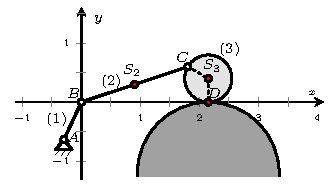
\includegraphics{abra1.pdf}} 
		\renewcommand{\thefigure}{\arabic{figure}} 
		\caption{Az ábrán 1 egység 0.1 méternek felel meg} 
	\end{figure}
	\newpage
	\feladat
	(2)-es test szögsebességének meghatározásához felírhatjuk egy \underline{pont} sebességét két oldalról, majd a két oldalt egyenlővé téve megoldhatjuk a kijövő egyenletrendszert.\\\\
	Legyen ez a \underline{pont} $\underline{S}_2$ súlypont. Ezt írjuk fel $\underline{v}_B$ majd $\underline{v}_C$ segítségével:\\\\
	\underline{v}_{\underline{S}_2} = \underline{v}_B + \underline{\omega}_2 \cross \underline{r}_{B\underline{S}_2}$ és \underline{v}_{\underline{S}_2} = \underline{v}_C + \underline{\omega}_2 \cross \underline{r}_{C\underline{S}_2}$
	\begin{figure}[h!] 
		\centering 
		\scalebox{2}{ 
			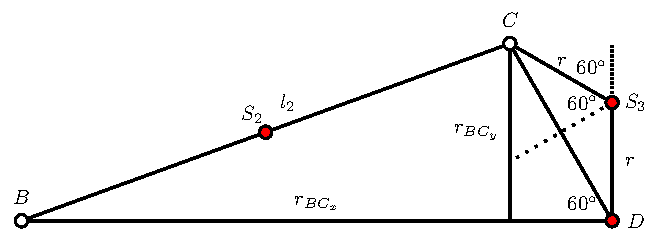
\includegraphics[width=150pt]{abra.2.pdf}} 
		\renewcommand{\thefigure}{\arabic{figure}} 
		\caption{Segítség a vektorok számításához} 
	\end{figure}\\
	Első egyenletet át tudjuk alakítani: \underline{v}_{\underline{S}_2} = \underline{v}_B + \underline{\omega}_2 \cross \underline{r}_{B\underline{S}_2} = \underline{v}_A + \underline{\omega}_1 \cross \underline{r}_{AB} + \underline{\omega}_2 \cross \underline{r}_{B\underline{S}_2}$, ahol:\\\\
	\underline{v}_A = \underline{0}$, \underline{A} \underline{pont} csuklós\hfill
	\underline{\omega}_1 = \begin{bmatrix}0\\0\\\omega_{1z}\end{bmatrix} \; \underline{\omega}_2 = \begin{bmatrix}0\\0\\\omega_{2}\end{bmatrix}$, síkmozgásról beszélünk\hfill
	\underline{r}_{AB} = \begin{bmatrix}l_1 \cdot \cos{\varphi}\\l_1 \cdot \sin{\varphi}\\0\end{bmatrix}\\\\\\
	\underline{r}_{B\underline{S}_2} = \dfrac{\underline{r}_{BC}}{2} = 0.5 \cdot \begin{bmatrix}\sqrt{l_2^2 - r_{BC_y}^2}\\\sin(60\fok) \cdot (2 \cdot \sin(60\fok) \cdot l_3)\\0\end{bmatrix}\\\\\\
	Második egyenletet át tudjuk alakítani: \underline{v}_{\underline{S}_2} = \underline{v}_C + \underline{\omega}_2 \cross \underline{r}_{C\underline{S}_2} = \underline{v}_D + \underline{\omega}_3 \cross \underline{r}_{DC} + \underline{\omega}_2 \cross \underline{r}_{C\underline{S}_2}$, ahol:\\\\
	\underline{v}_D = \underline{0}$, \underline{D} \underline{pont} gördül\hfill
	\underline{\omega}_2 = \begin{bmatrix}0\\0\\\omega_{2}\end{bmatrix} \; \underline{\omega}_3 = \begin{bmatrix}0\\0\\\omega_{3}\end{bmatrix}$, síkmozgásról beszélünk\hfill
	\underline{r}_{DC} = \begin{bmatrix}\dfrac{-r_{BC_y}}{\tan(60\fok)}\\r_{BC_y}\\0\end{bmatrix} \; \underline{r}_{C\underline{S}_2} = -\underline{r}_{B\underline{S}_2}$\\\\\\
	Ezek elvégzése után az \underline{x} és \underline{y} komponensekre kijött egyenleteket egymással egyenlővé tudjuk tenni:\\\\
	$-0.03 \cdot \omega_2 - 0.3172 = 0.03 \cdot \omega_2 - 0.06 \cdot \omega_3$\\\\
	$0.090139 \cdot \omega_2 + 0.1479 = -0.090139 \cdot \omega_2 - 0.034641 \cdot \omega_3$\\\\
	Az egyenletrendszer megoldása: \underline{\omega}_2 = \begin{bmatrix}0\\0\\-1.5404\end{bmatrix}\rads \quad \underline{\omega}_3 = \begin{bmatrix}0\\0\\3.7464\end{bmatrix}\rads\\\\\
	Így már csak vissza kell helyettesítenünk, hogy \underline{V}_{\underline{S}_2}-t megkapjuk:\\\\
	\underline{V}_{\underline{S}_2} = \begin{bmatrix}-0.271\\0.00907\\0\end{bmatrix}\ms \quad \abs{\underline{V}_{\underline{S}_2}} = 0.27115$
	\newpage
	\feladat
	Az előző feladatban felhasznált értékekkel vissza tudunk helyettesíteni, így:\\\\
	\underline{V}_{\underline{B}} = \begin{bmatrix}-0.317\\0.148\\0\end{bmatrix}\ms \quad \underline{V}_{\underline{S}_2} = \begin{bmatrix}-0.271\\0.00907\\0\end{bmatrix}\ms \quad \underline{V}_{\underline{C}} = \begin{bmatrix}-0.225\\-0.1298\\0\end{bmatrix}\ms\\\\\
	\underline{P}_2$ \underline{pont} megtalálásához pedig elegendő \underline{V}_{\underline{B}}$, \underline{V}_{\underline{S}_2}$ és \underline{V}_{\underline{C}}$ vektorokból merőlegest húzni, majd bejelölni metszéspontjukat.\\
	Ezt le is tudjuk ellenőrizni a következő számítással:\\\\
	\begin{figure}[h!] 
		\centering 
		\scalebox{2}{ 
			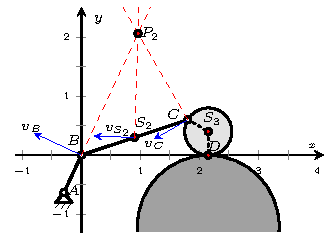
\includegraphics{abra3.pdf}} 
		\renewcommand{\thefigure}{\arabic{figure}} 
		\caption{Az ábrán 1 egység 0.5 m/s-nak felel meg} 
	\end{figure}
	\underline{r}_{B\underline{P}_2} = \dfrac{\underline{\omega}_2 \cross \underline{v}_{\underline{B}}}{\omega_2^2} = \begin{bmatrix}0.09603\\0.206\\0\end{bmatrix}\meter$
	\newpage
	\feladat
	(2)-es test szöggyorsulásának meghatározásához felírhatjuk egy \underline{pont} gyorsulását két oldalról, majd a két oldalt egyenlővé téve megoldhatjuk a kijövő egyenletrendszert.\\\\
	Legyen ez a \underline{pont} $\underline{S}_2$ súlypont. Ezt írjuk fel $\underline{a}_B$ majd $\underline{a}_C$ segítségével:\\\\
	\underline{a}_{\underline{S}_2} = \underline{a}_B + \underline{\varepsilon}_2 \cross \underline{r}_{B\underline{S}_2} - \omega_2^2 \cdot \underline{r}_{B\underline{S}_2}$ és \underline{a}_{\underline{S}_2} = \underline{a}_C + \underline{\varepsilon}_2 \cross \underline{r}_{C\underline{S}_2} - \omega_2^2 \cdot \underline{r}_{C\underline{S}_2}\\\\
	Első egyenletet át tudjuk alakítani:\\\underline{a}_{\underline{S}_2} = \underline{a}_B + \underline{\varepsilon}_2 \cross \underline{r}_{B\underline{S}_2} - \omega_2^2 \cdot \underline{r}_{B\underline{S}_2} = \underline{a}_A + \underline{\varepsilon}_1 \cross \underline{r}_{AB} - \omega_1^2 \cdot \underline{r}_{AB} + \underline{\varepsilon}_2 \cross \underline{r}_{B\underline{S}_2} - \omega_2^2 \cdot \underline{r}_{B\underline{S}_2}$, ahol:\\\\
	\underline{a}_A = \underline{0}$, mert kötött\hfill
	\underline{\varepsilon}_1 = \begin{bmatrix}0\\0\\0\end{bmatrix} = \underline{0}$, $\omega_1$ állandó\hfill\underline{\varepsilon}_2 = \begin{bmatrix}0\\0\\\varepsilon_{2}\end{bmatrix}$, síkmozgásról beszélünk\hfill
	\underline{r}_{AB}$, \underline{r}_{B\underline{S}_2}$, \underline{\omega}_1$, \underline{\omega}_2$ adottak\\\\\\
	Második egyenletet át tudjuk alakítani:\\\underline{a}_{\underline{S}_2} = \underline{a}_C + \underline{\varepsilon}_2 \cross \underline{r}_{C\underline{S}_2} - \omega_2^2 \cdot \underline{r}_{C\underline{S}_2} = \underline{a}_D + \underline{\varepsilon}_3 \cross \underline{r}_{DC} - \omega_3^2 \cdot \underline{r}_{DC} + \underline{\varepsilon}_2 \cross \underline{r}_{B\underline{S}_2} - \omega_2^2 \cdot \underline{r}_{B\underline{S}_2}$, ahol:\\\\
	\underline{\varepsilon}_2 = \begin{bmatrix}0\\0\\\varepsilon_2\end{bmatrix} = \underline{0} \quad \underline{\varepsilon}_3 = \begin{bmatrix}0\\0\\\varepsilon_3\end{bmatrix}$, síkmozgásról beszélünk\hfill
	\underline{r}_{DC}$, \underline{r}_{B\underline{S}_2}$, \underline{\omega}_2$, \underline{\omega}_3$ adottak\\\\\\
	\underline{a}_D = \begin{bmatrix}0\\a_{D_y}\\0\end{bmatrix}$ (körmozgásról beszélünk) $ = \underline{a}_{\underline{S}_3} + \underline{\varepsilon}_3 \cross \underline{r}_{\underline{S}_3D} - \omega_3^2 \cdot \underline{r}_{\underline{S}_3D} = \begin{bmatrix}0\\a_{\underline{S}_{3_y}} + \omega_3^2 \cdot l_3\\0\end{bmatrix}$, ahol:\\\\
	$S_{3_y} = - \dfrac{v_{\underline{S}_3}^2}{4 \cdot l_3}$ ($\underline{S}_3$ körpályán mozog) $ = \underline{v}_D + \underline{\omega}_3 \cross \underline{r}_{D\underline{S}_3}$\\\\
	Ezek elvégzése után az \underline{x} és \underline{y} komponensekre kijött egyenleteket egymással egyenlővé tudjuk tenni:\\\\
	$-1.003 = 0.03 \cdot \varepsilon_2 - 0.06 \cdot \varepsilon_3 + 0.7$\\\\
	$-1.509 = -0.0901 \cdot \varepsilon_2 - 0.02 \cdot 1.732 \cdot \varepsilon_3 - 0.3499$\\\\
	Az egyenletrendszer megoldása: \underline{\varepsilon}_2 = \begin{bmatrix}0\\0\\1.641\end{bmatrix}\radss \quad \underline{\varepsilon}_3 = \begin{bmatrix}0\\0\\29.2\end{bmatrix}\radss\\\\\
	Így már csak vissza kell helyettesítenünk, hogy \underline{V}_{\underline{S}_2}$-t megkapjuk:\\\\
	\underline{a}_{\underline{S}_2} = \begin{bmatrix}-1\\-1.51\\0\end{bmatrix}\ms \quad \abs{\underline{a}_{\underline{S}_2}} = 1.812$
	\newpage
	\feladat
	Az előző feladatban felhasznált értékekkel vissza tudunk helyettesíteni, így:\\\\
	\underline{a}_{\underline{B}} = \begin{bmatrix}-0.7396\\-1.586\\0\end{bmatrix}\mss \quad \underline{a}_{\underline{S}_2} = \begin{bmatrix}-1\\-1.51\\0\end{bmatrix}\mss \quad \underline{a}_{\underline{C}} = \begin{bmatrix}-1.266\\-1.433\\0\end{bmatrix}\ms\\\\\
	\underline{G}_2$ \underline{pont} megtalálásához pedig elegendő \underline{a}_{\underline{B}}$, \underline{a}_{\underline{S}_2}$ és \underline{a}_{\underline{C}}$ vektorokból merőlegest húzni, majd bejelölni metszéspontjukat.\\
	Ezt le is tudjuk ellenőrizni a következő számítással:\\\\
	\begin{figure}[h!] 
		\centering 
		\scalebox{1.2}{ 
			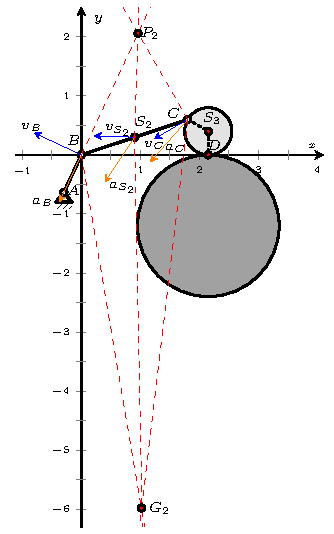
\includegraphics{abra4.pdf}} 
		\renewcommand{\thefigure}{\arabic{figure}} 
		\caption{Az ábrán 1 egység 3 m/s$^2$ felel meg} 
	\end{figure}
	\underline{r}_{\underline{S}_2\underline{G}_2} = \dfrac{\underline{\varepsilon}_2 \cross \underline{a}_{\underline{S}_2} + \omega_2^2 \cdot \underline{a}_{\underline{S}_2}}{\varepsilon_2^2 + \omega_2^4} = \begin{bmatrix}0.01171\\-0.628\\0\end{bmatrix}\meter$\\\\
	\feladat
	\underline{S}_2$ súlypont gyorsulásvektorának tangenciális és normális irányú komponenseihez először meg tudjuk határozni a tangenciális irányát és nagyságát, majd ebből a normálist is:\\\\
	\underline{e}_{\underline{S}_{2_t}} = \dfrac{\underline{v}_{\underline{S}_2}}{\abs{\underline{v}_{\underline{S}_2}}}$, mivel sebesség irányú\\\\
	\underline{a}_{\underline{S}_{2_t}} = (\underline{a}_{\underline{S}_2} \cdot \underline{e}_{\underline{S}_{2_t}}) \cdot \underline{e}_{\underline{S}_{2_t}}$ (így megvan a nagysága) $ = \begin{bmatrix}-0.951\\0.0318\\0\end{bmatrix}\mss \quad \abs{\underline{a}_{\underline{S}_{2_t}}} = 0.952$\\\\
	\underline{a}_{\underline{S}_{2_n}} = \underline{a}_{\underline{S}_2} - \underline{a}_{\underline{S}_{2_t}} = \begin{bmatrix}-0.0516\\-1.5411\\0\end{bmatrix}\mss \quad \abs{\underline{a}_{\underline{S}_{2_n}}} = 1.542$
	\begin{figure}[h!] 
		\centering 
		\scalebox{1.2}{ 
			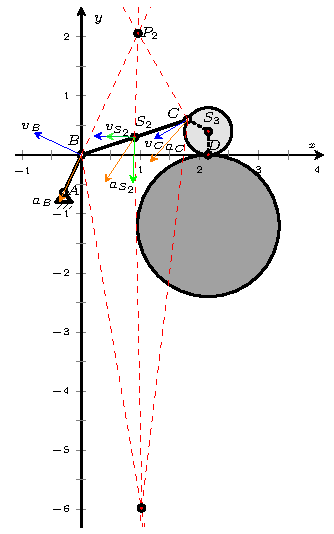
\includegraphics{abra5.pdf}} 
		\renewcommand{\thefigure}{\arabic{figure}} 
		\caption{Az ábrán zölddel jelölve \underline{a}_{\underline{S}_{2_n}}$ és \underline{a}_{\underline{S}_{2_t}}$} 
	\end{figure}
	\feladat 
	\underline{S}_2$ súlypont pályájának pillanatnyi görbületi sugarát könnyen meg tudjuk határozni:\\\\
	\abs{\underline{a}_{\underline{S}_{2_n}}} = \dfrac{\underline{v}_{\underline{S}_2}^2}{\rho_{\underline{S}_2}} \xrightarrow{} \rho_{\underline{S}_2} = 0.04768\meter$
\end{document}